\documentclass[sans,14pt]{beamer}
\usepackage{pgfpages}
%\setbeameroption{show notes on second screen}
%\setbeameroption{show notes}
\setbeameroption{hide notes}

\usepackage{etex}

\mode<presentation>
{
  \usetheme{Copenhagen}
  \usecolortheme{beaver}
  \usefonttheme[onlymath]{serif}
}

%% Change bullet points style
\setbeamertemplate{itemize items}{{\textemdash}}
\setbeamercolor*{item}{fg=MyDarkGrey}

%% Remove navigation symbols
\setbeamertemplate{navigation symbols}{}
\setbeamertemplate{headline}{}

%% Use only frame number (no total frame count) in footer
\setbeamertemplate{footline}{%
  \raisebox{5pt}{\makebox[\paperwidth]{\hfill\makebox[20pt]{
        \scriptsize\insertframenumber}}}
}

% Adjust margin of itemize environment
\setlength{\leftmargini}{0pt}
\setlength{\leftmarginii}{10pt}
\setlength{\leftmarginiii}{17pt}

%% Adjust font sizes
\setbeamerfont{frametitle}{size=\Large}
\setbeamerfont{normal text}{size=\small}
\setbeamerfont{itemize/enumerate body}{size=\small}
\setbeamerfont{itemize/enumerate subbody}{size=\small}
\setbeamerfont{itemize/enumerate subsubbody}{size=\footnotesize}

%%% To use the Cabin-Condensed fonts
%%% More fonts: see http://www.tug.dk/FontCatalogu
% \usepackage[latin1]{inputenc}
% \usepackage[T1]{fontenc}
% \usepackage[sfdefault]{cabin} 
\usepackage{PTSans} 
\usepackage{PTSansNarrow} 
\renewcommand*\familydefault{\sfdefault} %% Only if the base font of the document is to be sans serif
\usepackage[T1]{fontenc}

\newenvironment{ptnormal}{\fontfamily{PTSans-TLF}\selectfont}{\par}


\usepackage{amsmath}
\usepackage{amsfonts}
\usepackage{amssymb}
\usepackage{amsthm}
\usepackage{bm}
\usepackage{booktabs}
\usepackage{color}
\usepackage{epstopdf}
\usepackage{fancyhdr}
\usepackage{fancybox}
\usepackage{graphicx}
\usepackage{multirow}
\usepackage[normalem]{ulem}
\usepackage{url}
%


% tikzmark command, for shading over items
\usepackage{tikz}
\usetikzlibrary{calc}
\newcommand{\tikzmark}[1]{\tikz[overlay,remember picture] \node (#1) {};}
\usetikzlibrary{decorations.pathreplacing} % for curly braces
\usepackage[framemethod=tikz]{mdframed} % for fancy title page and other boxes

%% Subfigures
\usepackage[labelformat=simple,caption=false,textfont=scriptsize]{subfig}
\renewcommand{\thesubfigure}{\relax} % do not number captions of
                                     % subfloats



%%% Colors
%\usepackage{color}
\definecolor{MyBlue}{rgb}{0.27,0.62,0.73}%{0.,0.2,0.4} 
\definecolor{Aubergine}{rgb}{0.47,0.13,0.44} % 119 33 111
\definecolor{MyTurq}{rgb}{0.,0.8,0.8} 
\definecolor{MyDarkGrey}{rgb}{0.3,0.3,0.3} 
\definecolor{MyMedGrey}{rgb}{0.6,0.6,0.6} 
\definecolor{MyLightGrey}{rgb}{0.95,0.95,0.95} 
\definecolor{MyDarkRed}{rgb}{0.8,0.,0.} 
\definecolor{MyOrange}{rgb}{0.93,0.56,0.25}
\definecolor{MyPink}{rgb}{0.73,0.27,0.39}
\definecolor{MyLightYellow}{HTML}{FFFFCC}
%\usepackage[colorlinks=true,citecolor=MyTurq]{hyperref}
% \AtEveryCite{\color{MyMedGrey}}

\newcommand{\blue}[1]{{\color{MyBlue}{\textbf{#1}}}}
\newcommand{\red}[1]{{\color{MyOrange}{\textbf{#1}}}}
\newcommand{\black}[1]{{\color{MyDarkGrey}{\textbf{#1}}}}
\newcommand{\yellow}[1]{{\color{MyLightYellow}{\textbf{#1}}}}

\newcommand{\TODO}{{\color{MyDarkRed}{TODO~}}}

\setbeamercolor{normal text}{fg=MyDarkGrey}
\setbeamercolor{frametitle}{fg=Aubergine}

%%% ---- Titre des slides  (underline) ----------------
\setbeamertemplate{frametitle}{%
    \usebeamerfont{frametitle}\insertframetitle\strut%
    \vskip-.05\baselineskip%
    \leaders\vrule width \paperwidth\vskip1.pt%
    \vskip0pt%
    \nointerlineskip
}
%%% ---------------------------------------------------


% --- Math symbols -------------------------------------------------------------
\newcommand{\EE}{{\mathbb E}}
\newcommand{\PP}{{\mathbb P}}
\newcommand{\NN}{{\mathbb N}}
\newcommand{\RR}{{\mathbb R}}

\newcommand{\avec}{\vec{a}}
\newcommand{\alphavec}{\vec{\alpha}}
\newcommand{\betavec}{\vec{\beta}}
\newcommand{\cvec}{\vec{c}}
\newcommand{\fvec}{\vec{f}}
\newcommand{\muvec}{\vec{\mu}}
\newcommand{\rvec}{\vec{r}}
\newcommand{\thetavec}{\vec{\theta}}
\newcommand{\xvec}{\vec{x}}
\newcommand{\yvec}{\vec{y}}
\newcommand{\wvec}{\vec{w}}
\newcommand{\zvec}{\vec{z}}

% \newcommand{\amat}{{\mathbf A}}}
% \newcommand{\dmat}{{\mathbf D}}
% \newcommand{\gmat}{{\mathbf G}}
% \newcommand{\kmat}{{\mathbf K}}
% \newcommand{\lmat}{{\mathbf L}}
% \newcommand{\mmat}{{\mathbf M}}
% \newcommand{\wmat}{{\mathbf W}}
% \newcommand{\xmat}{{\mathbf X}}

\newcommand{\dset}{\mathcal{D}}
\newcommand{\fcal}{\mathcal{F}}
\newcommand{\ncal}{\mathcal{N}}
\newcommand{\rcal}{\mathcal{R}}
\newcommand{\sset}{\mathcal{S}}
\newcommand{\vset}{\mathcal{V}}
\newcommand{\tset}{\mathcal{T}}
\newcommand{\xcal}{\mathcal{X}}
\newcommand{\ycal}{\mathcal{Y}}

\newcommand{\lzeronorm}[1]{\left|\left|#1\right|\right|_0}
\newcommand{\lonenorm}[1]{\left|\left|#1\right|\right|_1}
\newcommand{\ltwonorm}[1]{\left|\left|#1\right|\right|_2}

\DeclareMathOperator*{\argmin}{arg\,min}
\DeclareMathOperator*{\argmax}{arg\,max}
% ------------------------------------------------------------------------------







\newcommand{\mytitle}{Bonnes pratiques}
\author{Chlo\'e-Agathe~Azencott}
\date{\small Juin 2024}

\begin{document}
{
  \begin{frame}[plain]
    \fontfamily{PTSansNarrow-TLF}\selectfont
    \begin{center}
      {\ptnormal{\textit{ECUE21.2 Science des données}}}
    \end{center}

    \vspace{100pt}

      {\Large \bf \mytitle}

      \insertauthor

      {\footnotesize
        \centerline{Center for Computational Biology (CBIO)}
      
        \centerline{Mines Paris PSL -- Institut Curie -- INSERM U900}

        \centerline{PSL Research University \& PR[AI]RIE, Paris, France}
      }

      \centerline {\insertdate}


      \vspace{-15pt}

      \begin{center}
        \begin{tabular}[b]{ccc}
          {\scriptsize \href{http://cazencott.info}{http://cazencott.info}} &
          {\scriptsize \href{chloe-agathe.azencott@minesparis.psl.eu}
            {chloe-agathe.azencott@minesparis.psl.eu}} & 
          {\scriptsize \href{https://lipn.info/@cazencott}{@cazencott@lipn.info}} \\
        \end{tabular}
      \end{center}
\end{frame}

% Do not count title slide when numbering frames
\addtocounter{framenumber}{-1}

\begin{frame}
  \begin{center}
    \Large 1. Visualisation de données
  \end{center}
\end{frame}

\begin{frame}
  \frametitle{1. Exemple 1}
  \begin{center}
    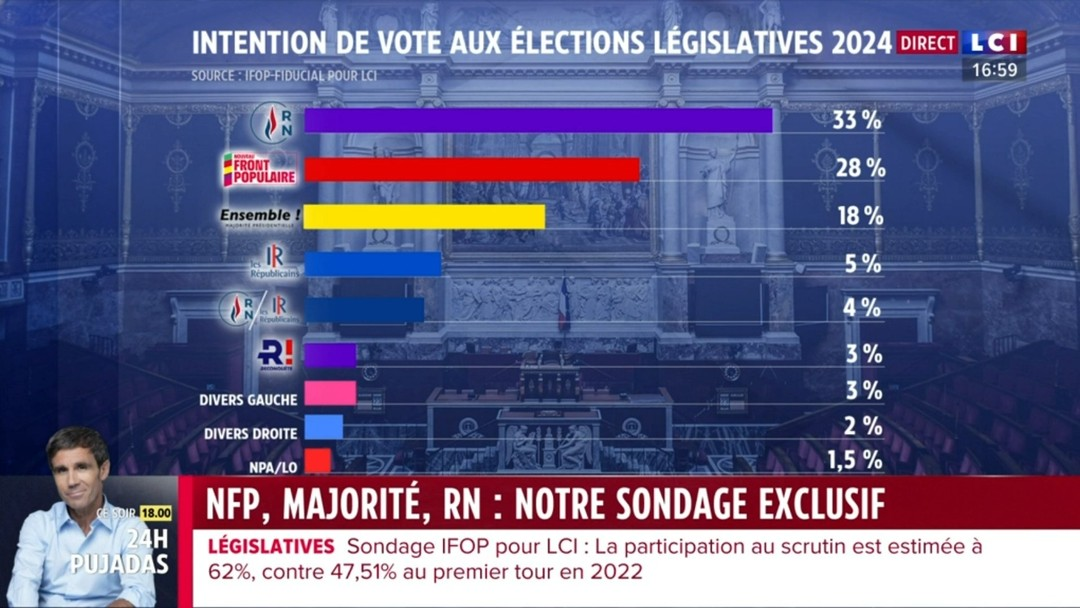
\includegraphics[width=\textwidth]{figures/jt_tf1_2024-06-17.png}
  \end{center}
  \begin{itemize}
  \item[] \footnotesize{TF1, 17 juin 2024, 16h56}
  \end{itemize}
\end{frame}

\begin{frame}
  \frametitle{1. Exemple 1}
  \begin{center}
    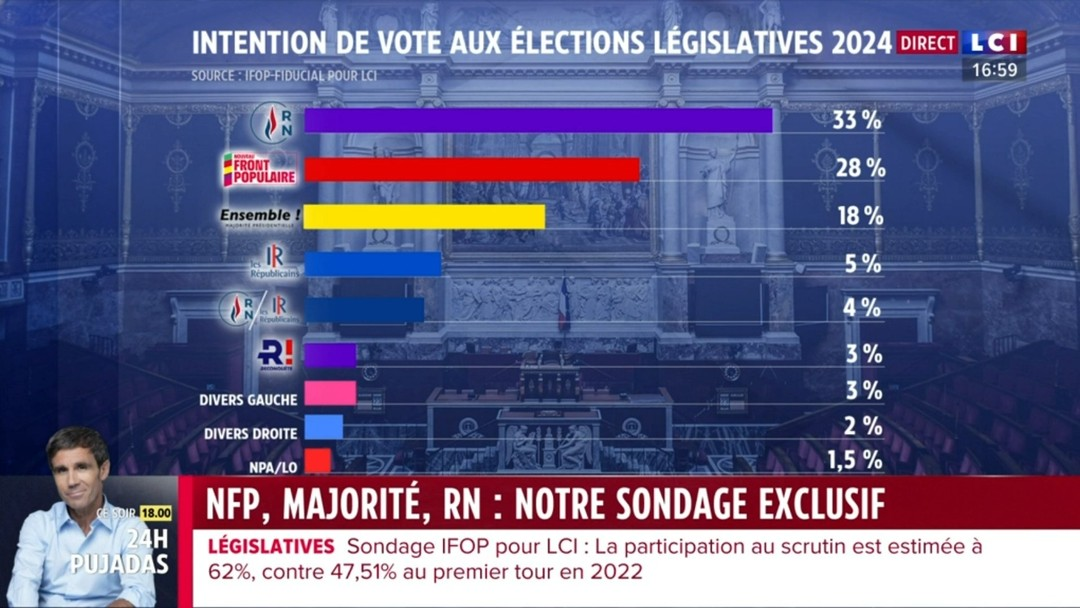
\includegraphics[width=0.5\textwidth]{figures/jt_tf1_2024-06-17.png}%
    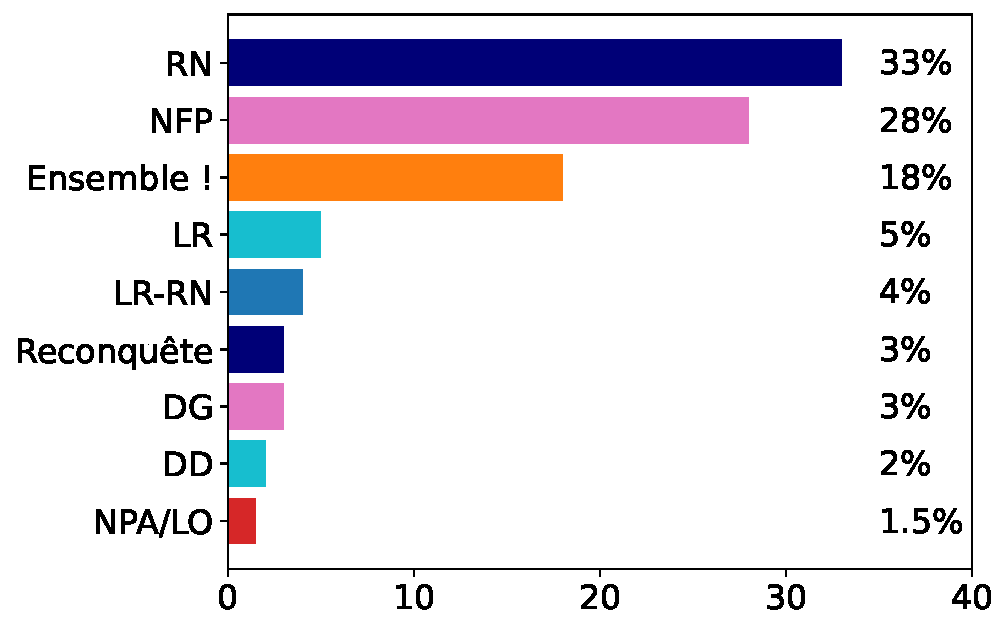
\includegraphics[width=0.5\textwidth]{figures/jt_tf1_2024-06-17_fixed.pdf}
  \end{center}
\end{frame}

\begin{frame}
  \frametitle{2. Exemple 2}
  \begin{itemize}
  \item[] Performance de 4 modèles sur un problème d'apprentissage
  \end{itemize}
  \begin{center}
    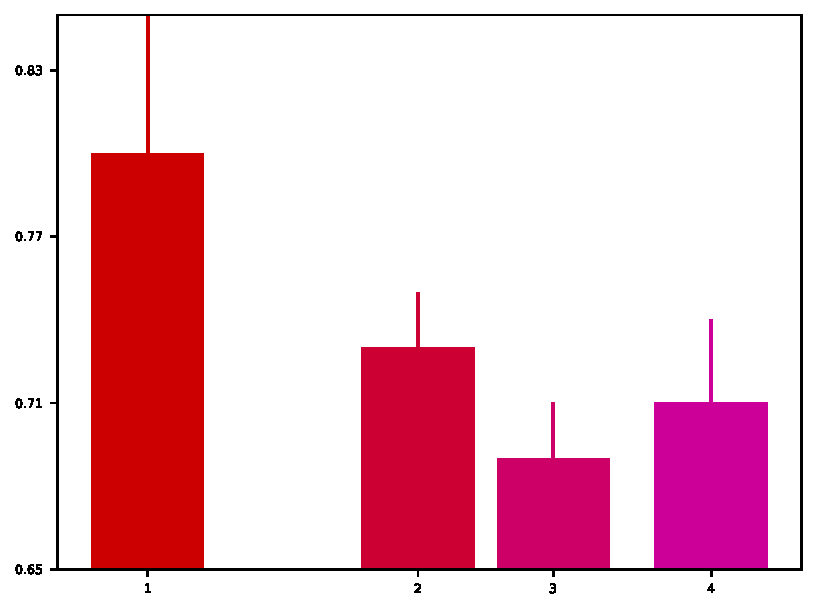
\includegraphics[width=0.8\textwidth]{figures/horrible_bar_plot}
  \end{center}
\end{frame}

\begin{frame}
  \frametitle{2. Exemple 2}
  \begin{itemize}
  \item[] Performance de 4 modèles sur un problème d'apprentissage
  \end{itemize}
  \begin{center}
    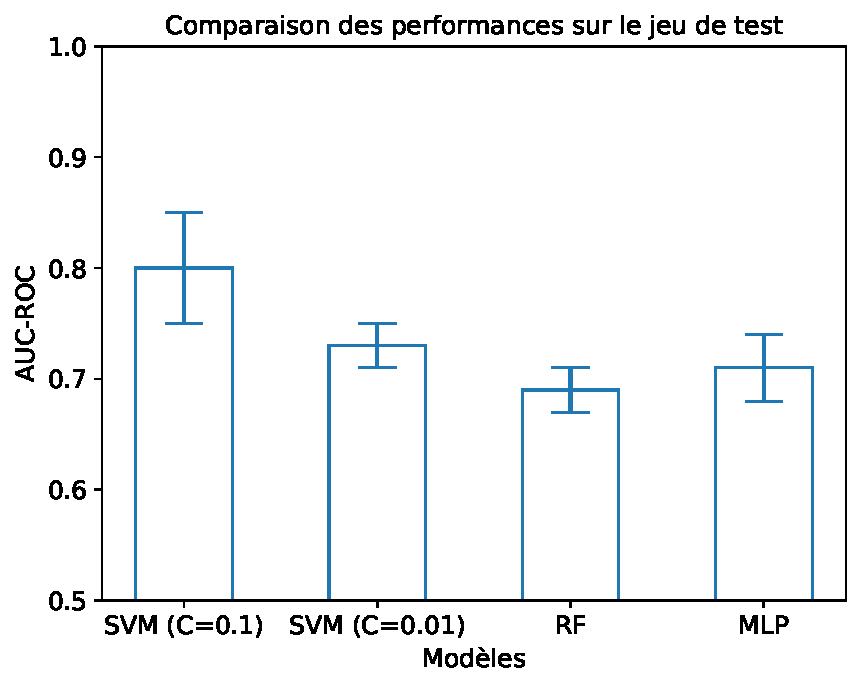
\includegraphics[width=0.8\textwidth]{figures/meilleur_bar_plot}
  \end{center}
\end{frame}

\begin{frame}
  \frametitle{3. Choix des axes (1)}
  \begin{minipage}[h]{0.49\linewidth}
    \begin{center}
      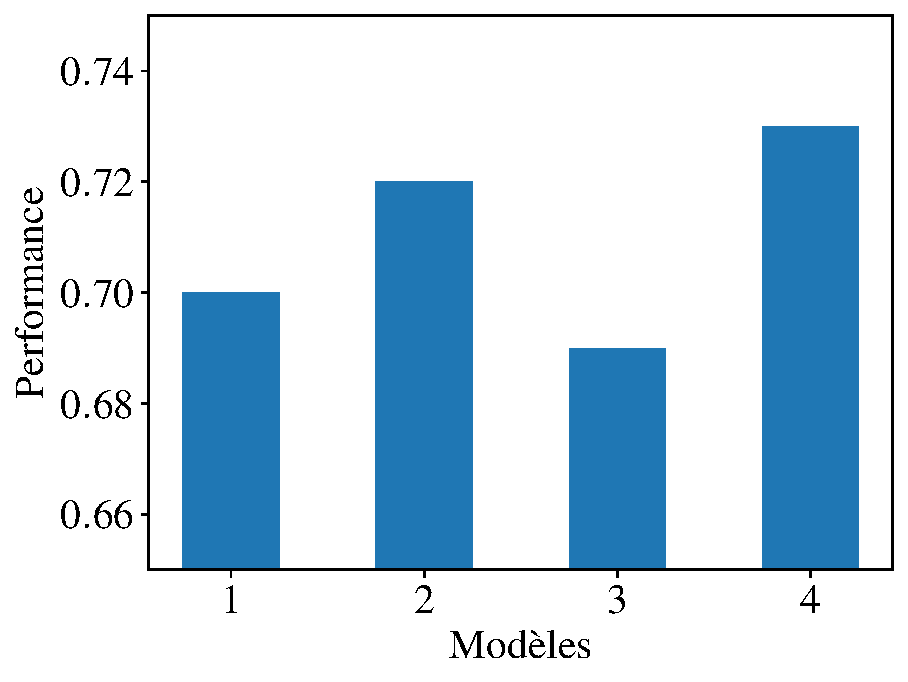
\includegraphics[width=\textwidth]{../poly/figures/pratiques/bars_start_nonzero}
    \end{center}
  \end{minipage}%
  \pause
  \hfill
  \begin{minipage}[h]{0.49\linewidth}
    \begin{center}
      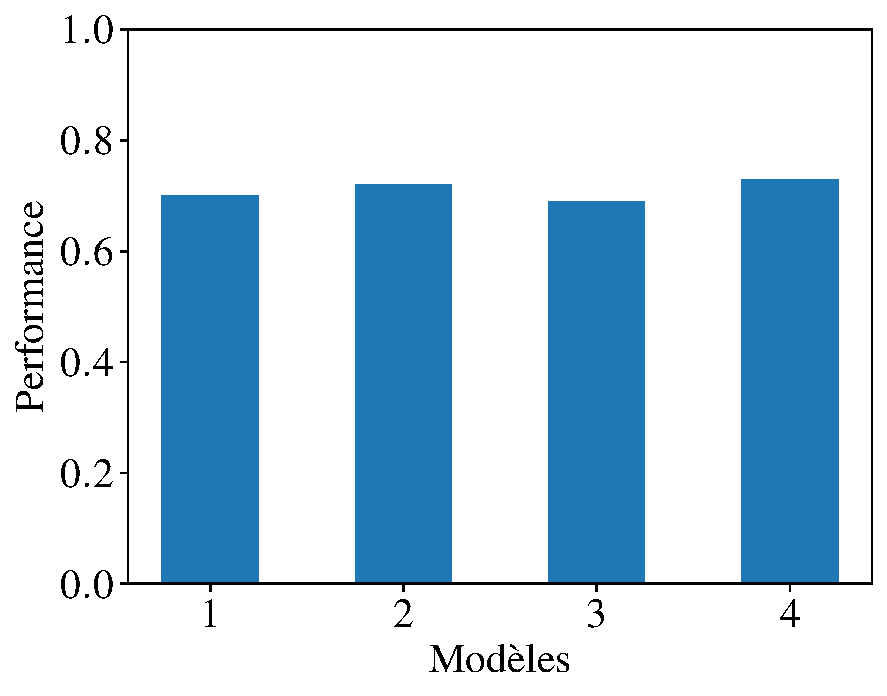
\includegraphics[width=\textwidth]{../poly/figures/pratiques/bars_start_zero}
    \end{center}
  \end{minipage}%
\end{frame}

\begin{frame}
  \frametitle{3. Choix des axes (2)}
  \begin{minipage}[h]{0.49\linewidth}
    \begin{center}
      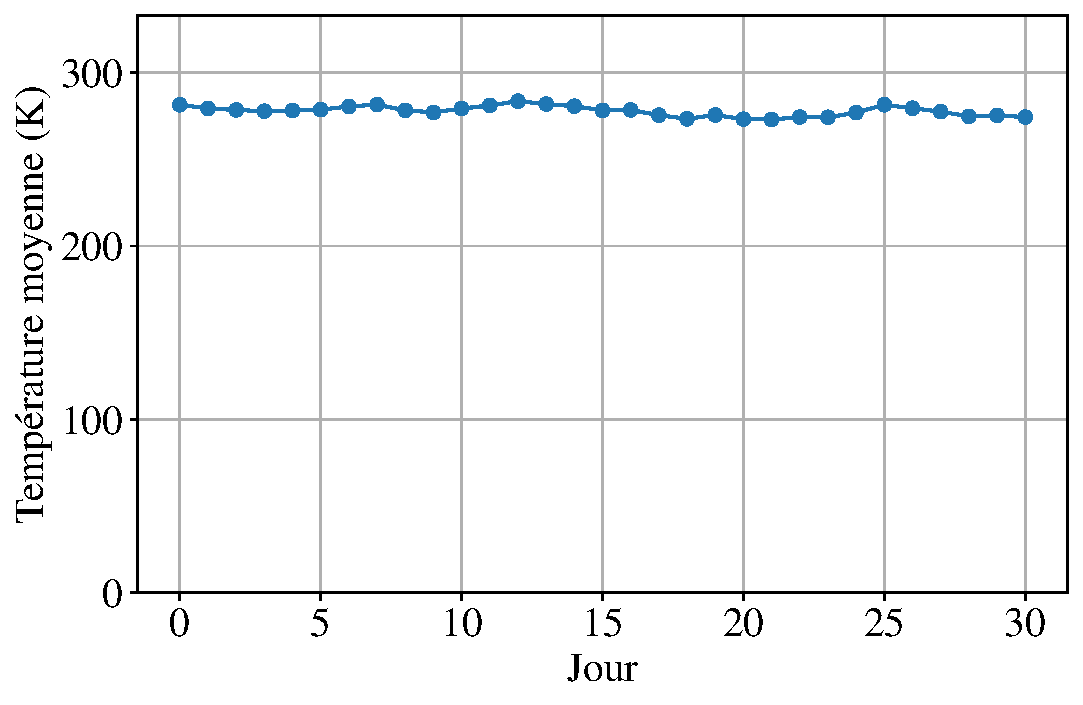
\includegraphics[width=\textwidth]{../poly/figures/pratiques/line_start_zero}
    \end{center}
  \end{minipage}%
  \pause
  \hfill
  \begin{minipage}[h]{0.49\linewidth}
    \begin{center}
      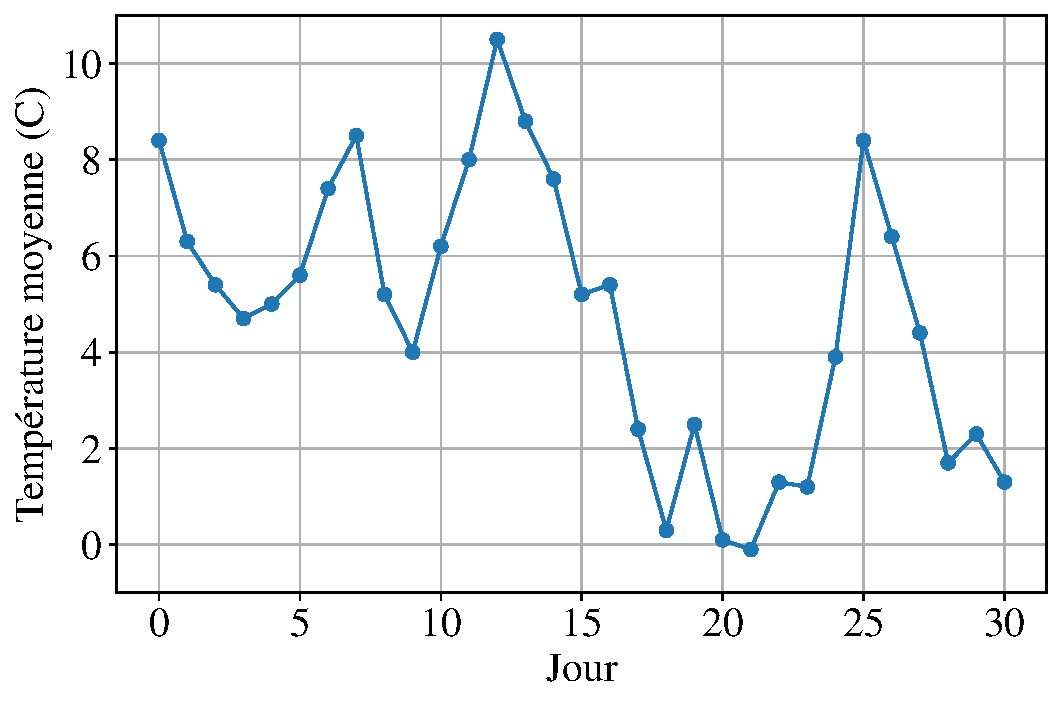
\includegraphics[width=\textwidth]{../poly/figures/pratiques/line_start_nonzero}
    \end{center}
  \end{minipage}%
\end{frame}

\begin{frame}
  \frametitle{4. Proportional ink}
  \begin{minipage}[h]{0.49\linewidth}
    \begin{center}
      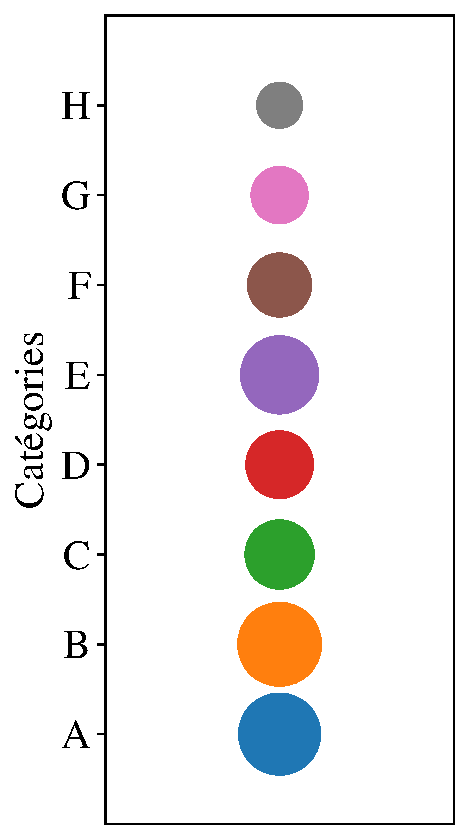
\includegraphics[width=0.45\textwidth]{../poly/figures/pratiques/areas_bubbles}
    \end{center}
  \end{minipage}%
  \hfill
  \pause
  \begin{minipage}[h]{0.49\linewidth}
    \begin{center}
      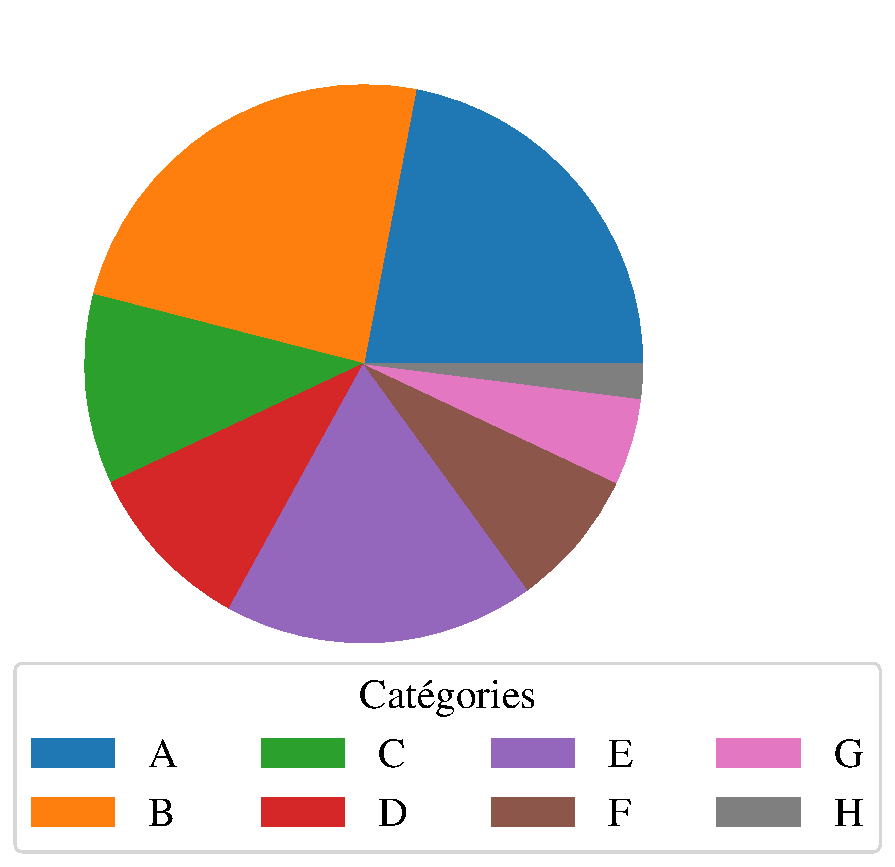
\includegraphics[width=0.9\textwidth]{../poly/figures/pratiques/areas_pie}
    \end{center}
  \end{minipage}
  \pause
  \begin{minipage}[h]{0.49\linewidth}
    \begin{center}
      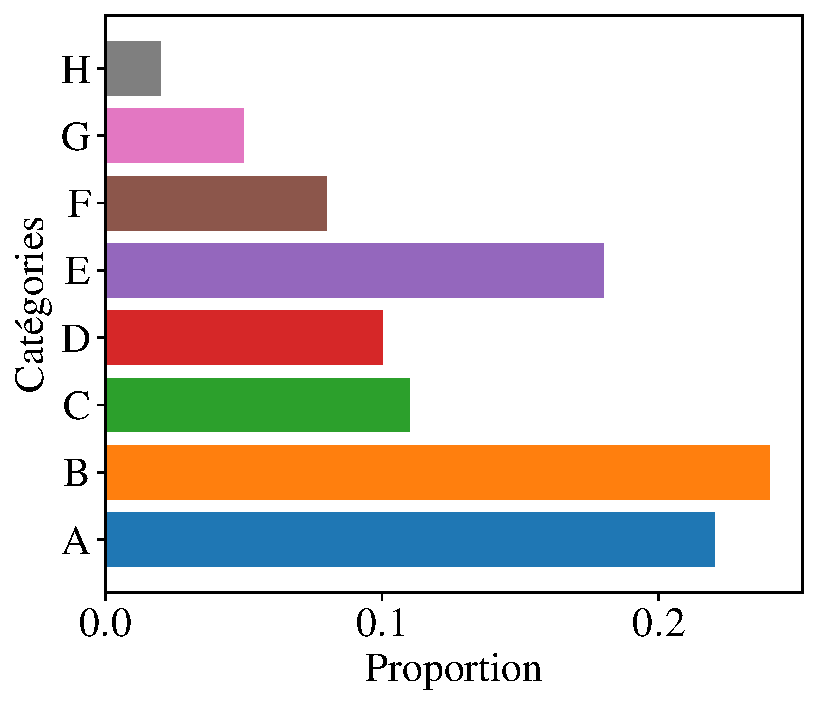
\includegraphics[width=0.8\textwidth]{../poly/figures/pratiques/areas_bars}
    \end{center}
  \end{minipage}  
\end{frame}


\begin{frame}
  \frametitle{5. Dyschromatopie}
  \begin{minipage}[h]{0.49\linewidth}
    \begin{center}
      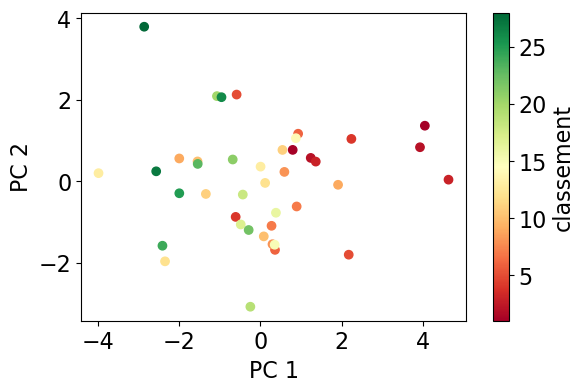
\includegraphics[width=\textwidth]{figures/pca_plot_RdYlGn} \newline
      {\footnotesize{\texttt{plt.scatter(\dots cmap='RdYlGn')}}}
    \end{center}
  \end{minipage}%
  \pause
  \hfill
  \begin{minipage}[h]{0.49\linewidth}
    \begin{center}
      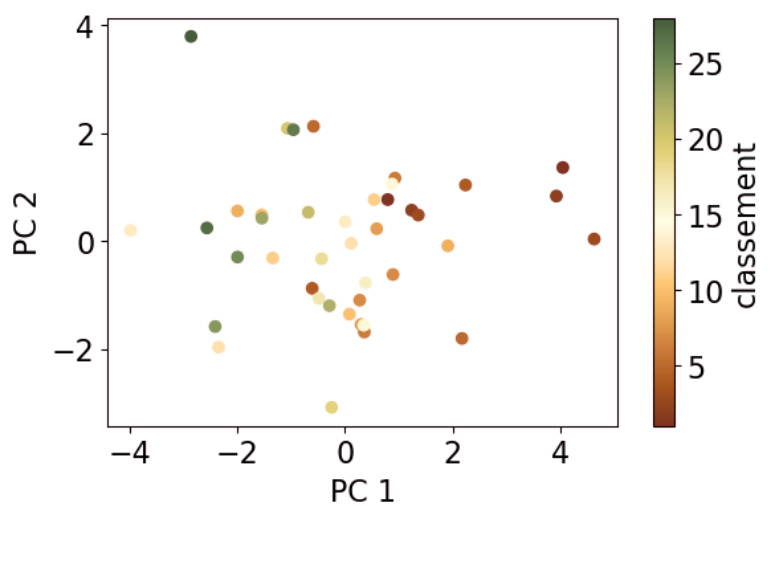
\includegraphics[width=\textwidth]{figures/pca_plot_RdYlGn_coblis} \newline
      {\footnotesize{Simulation de deutéranopie par CoBliS}}
      \end{center}
    \end{minipage}%
    \vspace{2em}
    \begin{itemize}
    \item[] \footnotesize \hfill [\href{https://www.color-blindness.com/coblis-color-blindness-simulator/}{lien vers CoBliS}]
    \end{itemize}
\end{frame}

\begin{frame}
  \frametitle{5. Dyschromatopie}
  \begin{minipage}[h]{0.49\linewidth}
    \begin{center}
      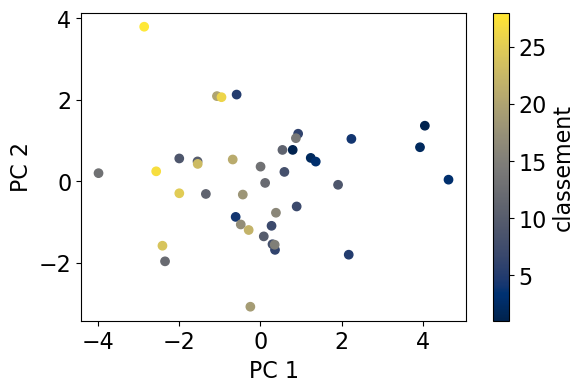
\includegraphics[width=\textwidth]{figures/pca_plot_cividis} \newline
      {\footnotesize{\texttt{plt.scatter(\dots cmap='cividis)}}}
    \end{center}
  \end{minipage}%
  \pause
  \hfill
  \begin{minipage}[h]{0.49\linewidth}
    \begin{center}
      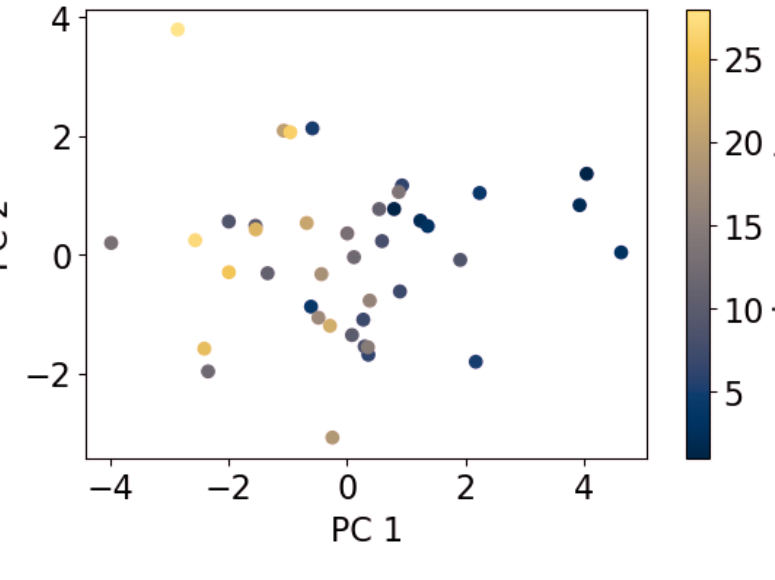
\includegraphics[width=\textwidth]{figures/pca_plot_cividis_coblis} \newline
      {\footnotesize{Simulation de deutéranopie par CoBliS}}
      \end{center}
    \end{minipage}%
    \vspace{2em}
    \begin{itemize}
    \item[] \footnotesize \hfill [\href{https://www.color-blindness.com/coblis-color-blindness-simulator/}{lien vers CoBliS}]
    \end{itemize}
\end{frame}


\begin{frame}
  \begin{center}
    \Large 2. Questionnements autour de l'utilisation du ML
  \end{center}
\end{frame}


\begin{frame}
  \begin{center}
    \Large 2.1 Quel problème ?
  \end{center}
\end{frame}

\begin{frame}[t]
  \frametitle{Exemple : Détection de criminels}
  \begin{itemize}
  \item Article sur arxiv : \textit{Automated Inference on Criminality using
      Face Images}, Xiaolin Wu \& Xi Zhang (2017)
  \item Motivation : \textcolor{MyBlue}{``Unlike a human examiner/judge, a
      computer vision classifier has absolutely no subjective baggage, having
      no emotions, no biases whatsoever due to past experience, race, religion,
      political doctrine, gender, age, etc.''}
  \end{itemize}
\end{frame}


\begin{frame}
  \begin{center}
    \Large 2.2 Quelles donnéees ?
  \end{center}
\end{frame}

\begin{frame}[t]
  \frametitle{Exemple : Détection de criminels}
  \begin{itemize}
  \item Article sur arxiv : \textit{Automated Inference on Criminality using
      Face Images}, Xiaolin Wu \& Xi Zhang (2017)
  \end{itemize}
  \begin{center}
    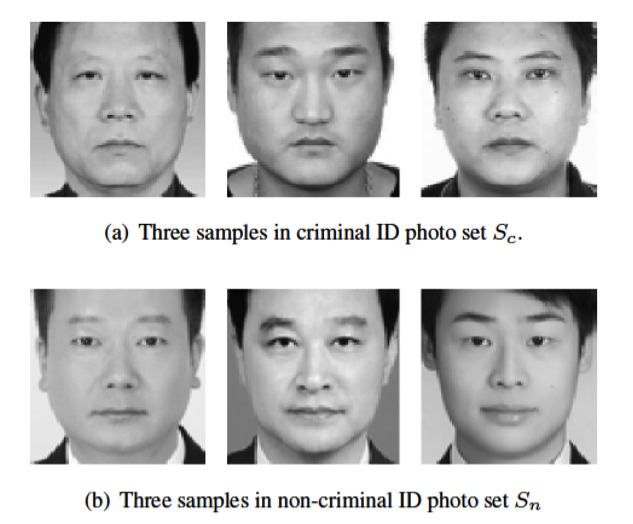
\includegraphics[width=0.6\textwidth]{figures/criminals_wu_zhang_2016} \\
    \footnotesize Figure 1. Sample ID photos in our data set.
  \end{center}
\end{frame}


\begin{frame}[t]
  \frametitle{Exemple : Recrutement automatisé}
  \begin{itemize}
  \item[] {\footnotesize \hfill source: Reuters [\href{https://www.reuters.com/article/us-amazon-com-jobs-automation-insight-idUSKCN1MK08G}{lien}]}
  \item Système fortement biaisé en faveur des CV déposés par des hommes
  \item Pourtant cette information ne faisait pas partie des variables utilisées
    \vfill
  \end{itemize}
\end{frame}


\begin{frame}
  \frametitle{It's not just AI : oxymètres de pouls}
  \begin{itemize}
  \item {\textit{Racial Bias in Pulse Oximetry Measurement}}, Sjoding et al., New
    England Journal of Medicine, 2020; 383:2477-2478 \href{https://www.nejm.org/doi/full/10.1056/NEJMc2029240}{[lien]}
  \end{itemize}
  \begin{center}
    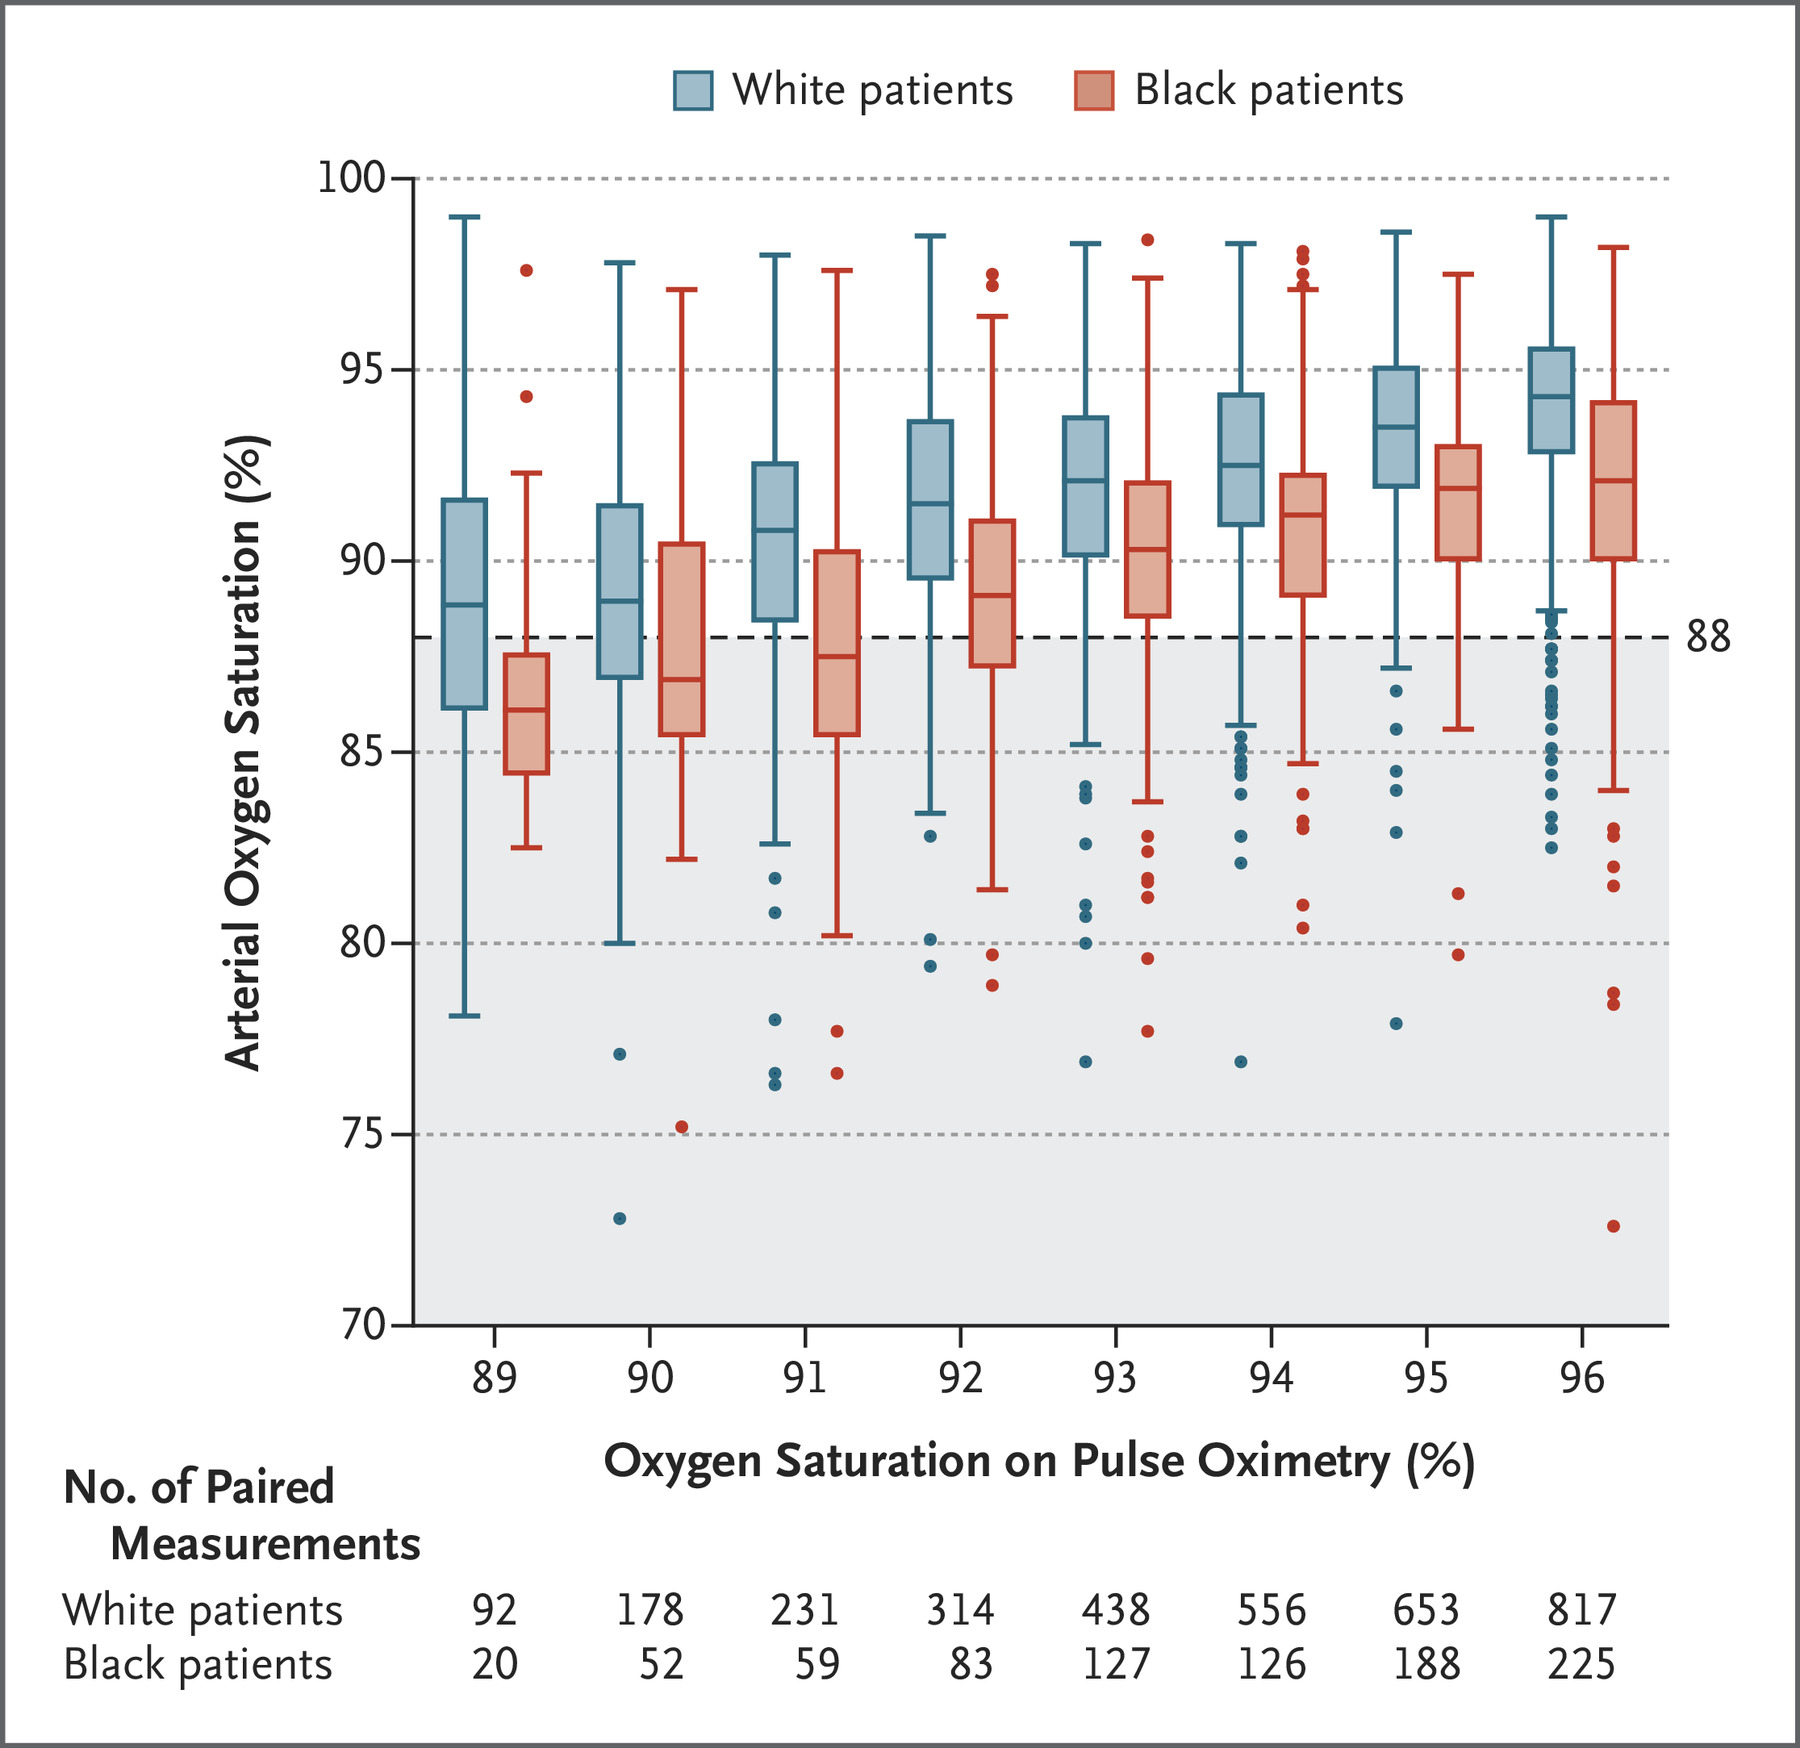
\includegraphics[width=0.6\textwidth]{figures/nejmc_sjoding2020} \\
    \footnotesize Accuracy of Pulse Oximetry in Measuring Arterial Oxygen
    Saturation, According to Race.
  \end{center}
\end{frame}

\begin{frame}
  \frametitle{Acquisition des données}
\end{frame}


% \begin{frame}
%   \begin{center}
%     \Large 2. Équité des algorithmes
%   \end{center}
% \end{frame}

% \begin{frame}[t]
%   \frametitle{1. Recrutement automatisé (Amazon)}
%   \begin{itemize}
%   \item[] {\footnotesize \hfill source: Reuters [\href{https://www.reuters.com/article/us-amazon-com-jobs-automation-insight-idUSKCN1MK08G}{lien}]}
%   \item Système fortement biaisé en faveur des CV déposés par des hommes
%   \item Pourtant le sexe ne faisait pas partie des variables utilisées
%     \vfill
%   \end{itemize}
% \end{frame}

% \begin{frame}[t]
%   \frametitle{2. Détection de criminels par leur photo}
%   \begin{itemize}
%   \item Article sur arxiv : \textit{Automated Inference on Criminality using
%       Face Images}, Xiaolin Wu \& Xi Zhang (2017)
%   \item Motivation : \textcolor{MyBlue}{``Unlike a human examiner/judge, a
%       computer vision classifier has absolutely no subjective baggage, having
%       no emotions, no biases whatsoever due to past experience, race, religion,
%       political doctrine, gender, age, etc.''}
%   \end{itemize}
% \end{frame}


\begin{frame}
  \begin{center}
    \Large 4. Fiabilité
  \end{center}
\end{frame}

\begin{frame}
  \frametitle{Attaque (bruit gaussien)}
  \begin{center}
    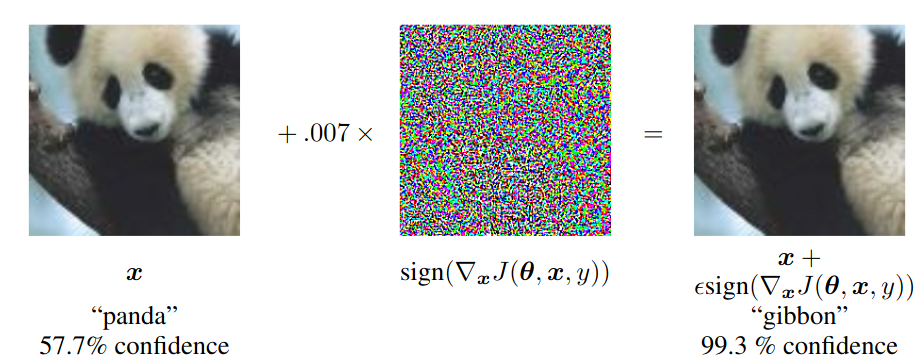
\includegraphics[width=\textwidth]{figures/adversarial_goodfellow_2015.png} \\
    {\footnotesize Goodfellow, Shlens \& Szegedy (ICLR 2015)}
  \end{center}
\end{frame}

\begin{frame}
  \frametitle{Attaque (1-pixel)}
  \begin{center}
    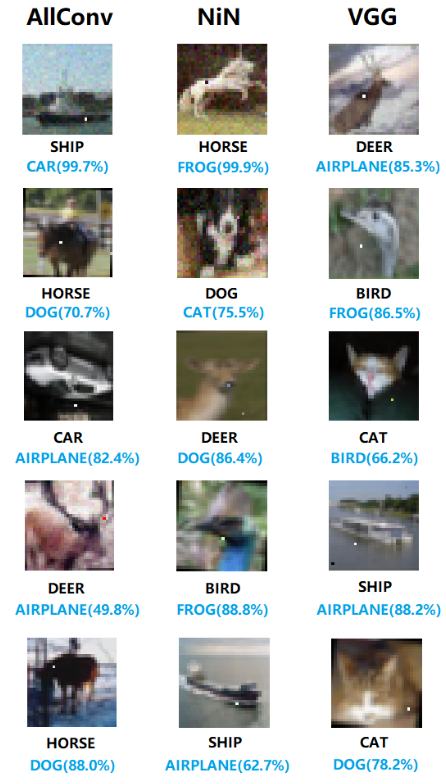
\includegraphics[width=0.35\textwidth]{figures/adversarial_su_2019.png} \\
    {\footnotesize Su, Vargas \& Kouichi (IEEE Transactions on Evolutionary Computation 2019)}
  \end{center}
\end{frame}

\begin{frame}
  \frametitle{Attaque (monde réel)}
  \begin{center}
    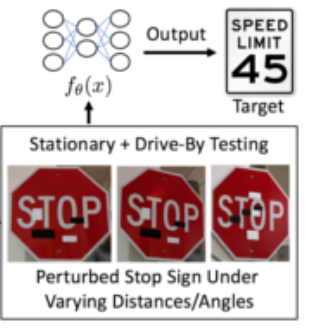
\includegraphics[width=0.4\textwidth]{figures/adversarial_eykholt_2018.png} \\
    {\footnotesize Eykholt et al. (CBPR 2018)}
  \end{center}
\end{frame}

\begin{frame}[t]
  \frametitle{EchoLeak (juin 2025)}
  
  \begin{itemize}
  \item[] {\footnotesize \hfill source: AIM Labs \href{https://www.aim.security/lp/aim-labs-echoleak-blogpost}{(lien)}}
  \item \black{Injection:} Attacker sends innocuous-looking email that includes LLM scope violation exploit
  \item \black{Action:} User asks Copilot a question 
  \item \black{Scope Violation:} Copilot mixes attacked input with sensitive data
  \item \black{Retrieval:} Copilot leaks sensitive data to attacker via SharePoint URLs
  \end{itemize}
\end{frame}


\begin{frame}
  \begin{center}
    \Large 5. Ressources
  \end{center}
\end{frame}



\end{document}

%%% Local Variables:
%%% mode: latex
%%% TeX-master: t
%%% End:
